% Beginning of a chapter
% Use labels for referencing
\chapter{Movement patterns}\label{movementpatterns} 
\section{Introduction}\label{intro}
% this is a comment
% normal text
Lorem ipsum dolor sit amet, consectetur adipiscing elit. Cras placerat dolor at nibh dapibus condimentum. Aenean hendrerit libero eget leo consequat varius. Nullam in mollis purus. Vestibulum id interdum magna. Aliquam a ex dolor. Pellentesque nec dolor lorem. Nunc condimentum ac diam vitae rutrum. Quisque vulputate lobortis varius. In interdum dolor justo, eget laoreet leo pretium sit amet. \\ % newline
Lorem ipsum dolor sit amet, consectetur adipiscing elit. In tincidunt cursus massa ullamcorper placerat. Suspendisse eu justo lorem. Aliquam erat volutpat. Etiam neque enim, gravida id luctus nec, semper id felis. Sed dolor orci, consectetur id consectetur nec, rutrum vitae quam. Duis vel lobortis nisi. Suspendisse vel nibh ut est aliquam sollicitudin id quis odio. Nunc accumsan at massa ac interdum. Donec sit amet sem eu nibh imperdiet accumsan a eu risus. Nam euismod elit nec elit blandit, sed condimentum augue dapibus. Nulla fermentum velit sit amet tincidunt mattis. \\
Vivamus ut nulla id nisl imperdiet vulputate. Duis ornare egestas neque, porttitor fringilla dui iaculis imperdiet. Nulla facilisi. Sed odio diam, tempor eu metus a, laoreet feugiat tellus.\\
Begin numbered list
\begin{enumerate}
\item number 1
\item number 2
\item number 3
\item number 4
\end{enumerate}
Begin bullet list
\begin{itemize}
\item this is a bullet
\item this as well
\end{itemize}


\section{Include graphics}
To include graphics in the document, use the following template:

\begin{figure}[H]
\centering
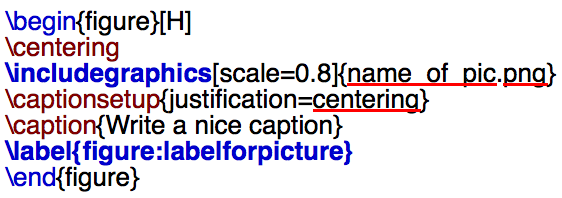
\includegraphics[scale=0.8]{name_of_pic.png}
\captionsetup{justification=centering}
\caption{Write a nice caption}
\label{figure:labelforpicture}
\end{figure}

If you want to refer to a picture (or section/chapter/whatever) in the text, this can be done using the 'autoref' function. \autoref{figure:labelforpicture} shows how to include graphics in a document. This also works for sections: \autoref{movementpatterns}.

\section{Tables}
Use \url{http://www.tablesgenerator.com} for creating nice looking tables. Use the 'booktabs' style!!!
\begin{table}[H]
\centering
\caption{My caption}
\label{my-label}
<<<<<<< HEAD
\begin{tabular}{lll}[H]
\hline
this & is      & a      \\ \hline
=======
\begin{tabular}{@{}lll@{}}
\toprule
this & is      & a      \\ \midrule
>>>>>>> 3dc9814e185ffebcba50bc64c0886fdaf49dc3d0
nice & looking & table  \\
am   & i       & right? \\ \bottomrule
\end{tabular}
\end{table}
Unfortunately, LaTeX always places tables at the top or bottom of a page, so it will mostly mess up the layout! Use proper referencing in the text to make sure tables are read as they should! \autoref{my-label}.

\section{Referencing}
It would be nice if everyone could go over the parts they have written in the mid-term review and find everything they have referenced. You can easily import biblatex styled references from google scholar. If you search in google scholar for a title, there is usually a link below the result, 'cite'. Then you can select 'bibtex' as an option to download a file. The text inside this file can be copied into the 'report.bib' file. If you want to cite an author, that can be done using the 'cite' option. i.e. this author was used in the mid term review:
Let's cite! The Einstein's journal paper \cite{mautz2012indoor} and the Dirac's 
book \cite{meneses2012large} are physics related items. 

\section{bold and italics}
\textbf{this text will be bold!}
\textit{this text will be in italics}




